\section{Test with Users}
\label{sec:test}

\subsection{Experiment Design}
The experiments we performed have two parts:\\

\begin{itemize}
	\item \textbf{Gesture Control and Collision Avoidance}: To test this part the tester has to teleoperate MASHI using our gesture control system and perform some simple tasks, going out of the laboratory room and coming back. The testers are also asked to try to collide and interact with the environment so they could test the effectiveness of the collision system. After the test the tester has to answer a short survey about the user friendliness and the efficiency of our system.
	
	\item \textbf{Vital Space}: In the second and last part of the test we focus on the personal distance the users feel good interacting with the robot. We ask the users what is the distance to the robot they feel comfortable with and try approaching the robot to them.
\end{itemize}

The small survey consists of the following 10 questions:

\begin{enumerate}
	\item The system is easy to use. (Disagree 1 to 5 Totally Agree)
	\item The system is intuitive. (Disagree 1 to 5 Totally Agree)
	\item The system responds accordingly to your expectations. (Disagree 1 to 5 Totally Agree)
	\item What would you improve from the system?
	\item The gesture commands are easy and intuitive. (Disagree 1 to 5 Totally Agree)
	\item Which gesture is more complicated to detect?
	\item Which improvement do you think would be interesting for the gesture control?
	\item The anti-collision system is useful. (Disagree 1 to 5 Totally Agree)
	\item Do you think the speed reduction is useful?
	\item After the test, at which distance you consider the robot must stop in order to avoid a collision with a human?
\end{enumerate}





\subsection{Experiment Results}

Given the duration of the test, around 20 minutes, we performed the test with only 4 users, we can see some pictures of the testing session in the Figures \ref{fig:gest}, \ref{fig:comf}, \ref{fig:coll}. The number of users is not enough to do any significant statistical analysis but we can have an idea of what are the weak and the strong points of our system.\\

\begin{figure}[htb!]
	\centering
	\begin{subfigure}[b]{0.3\textwidth}
		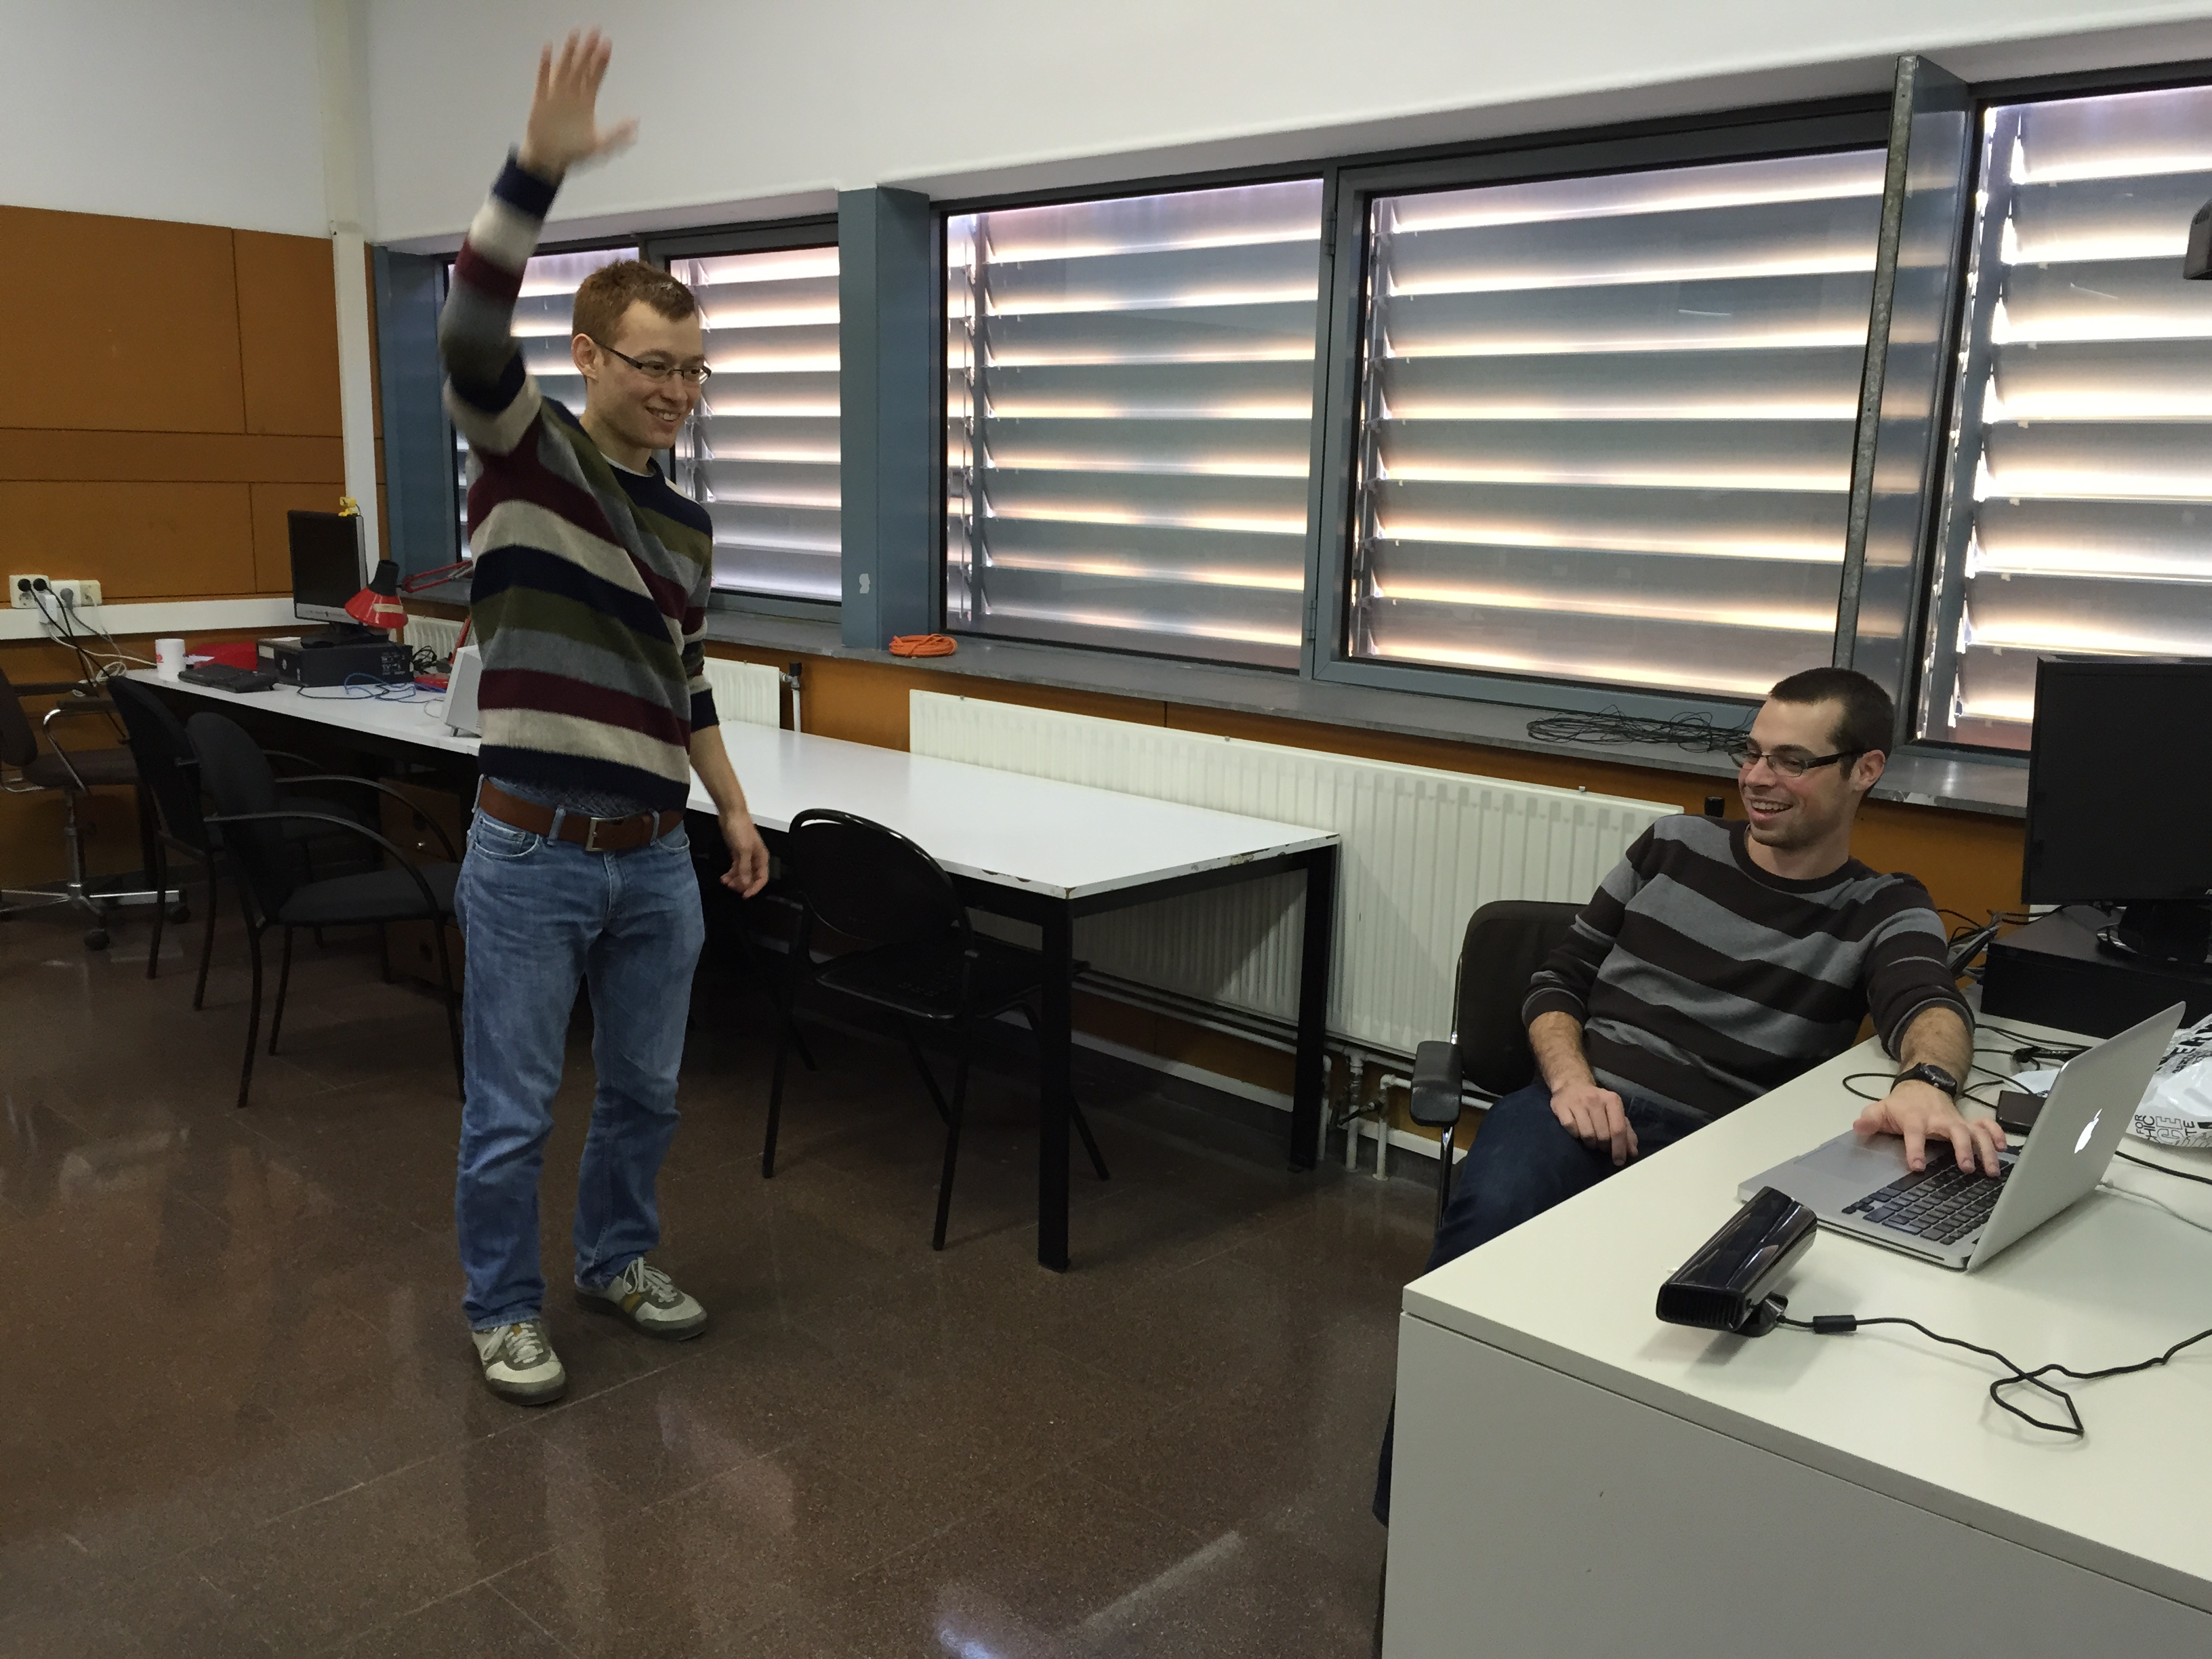
\includegraphics[width=\textwidth]{images/2_Gestures_Test.JPG}
		%\caption{Gestures Test}
		\label{fig:gest1}
	\end{subfigure}%
	~ %add desired spacing between images, e. g. ~, \quad, \qquad, \hfill etc.
	%(or a blank line to force the subfigure onto a new line)
	\begin{subfigure}[b]{0.3\textwidth}
		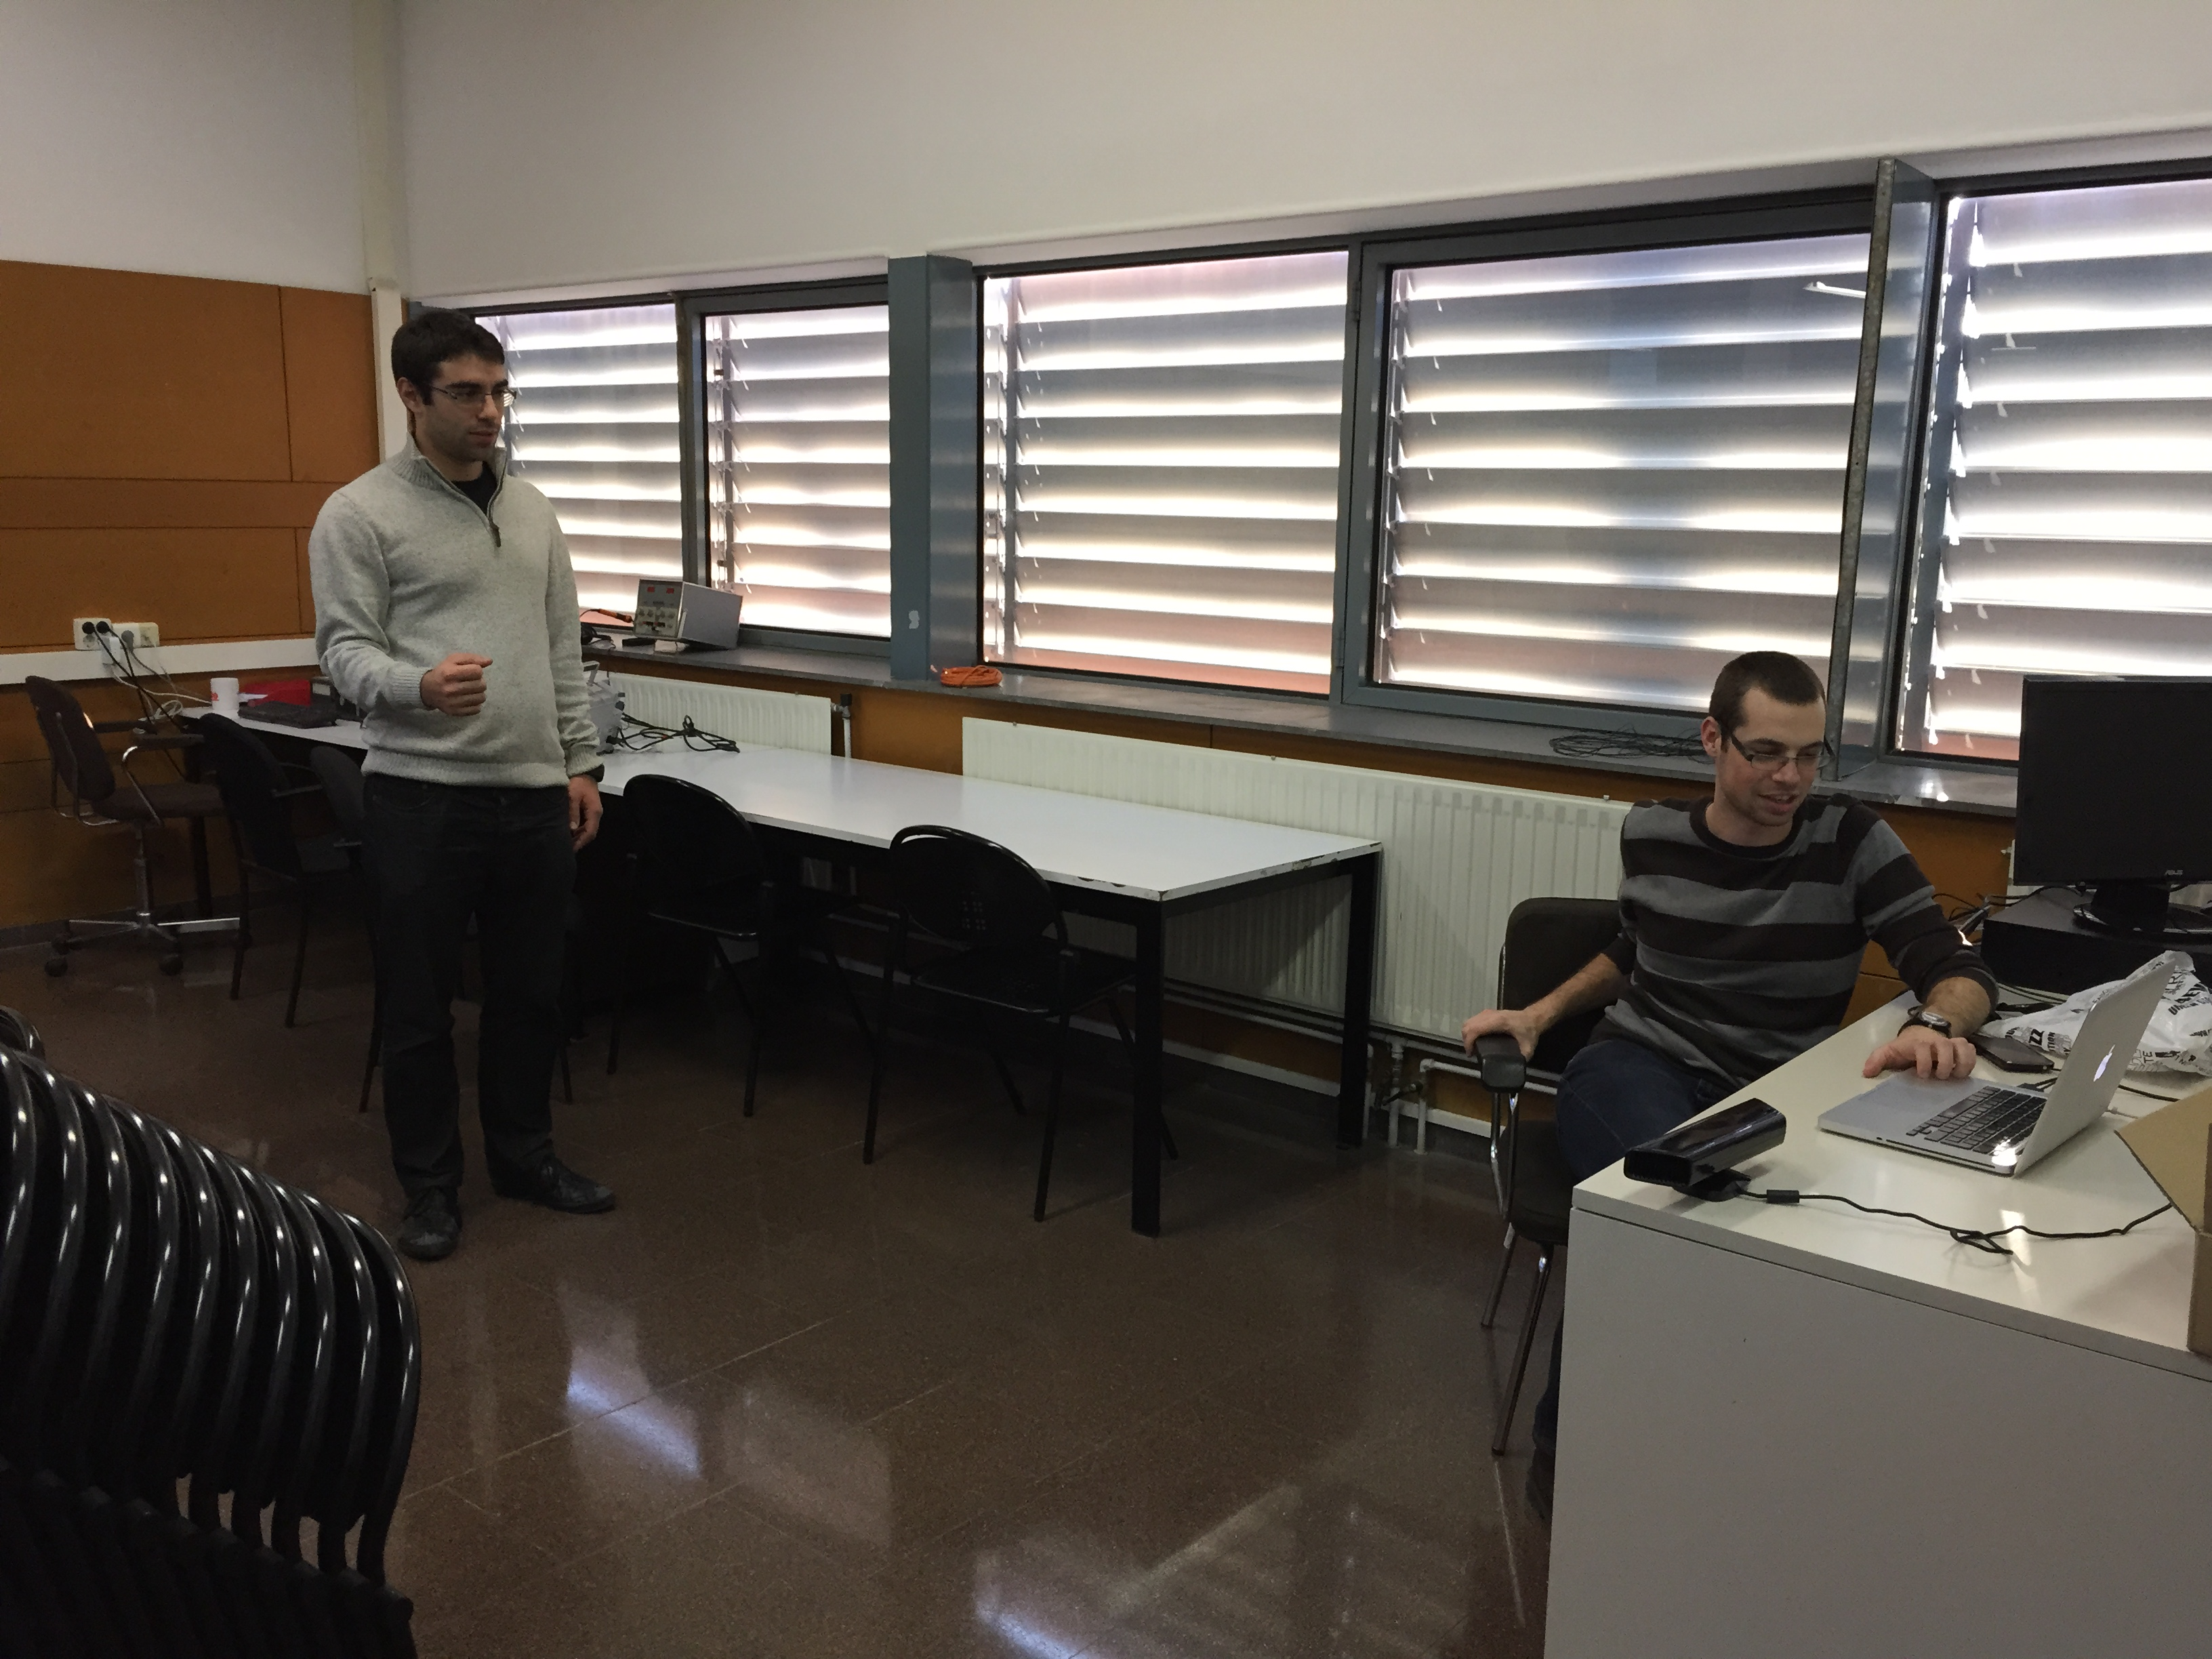
\includegraphics[width=\textwidth]{images/3_Gestures_Test.JPG}
		%\caption{Gestures Test}
		\label{fig:gest2}
	\end{subfigure}
	~ %add desired spacing between images, e. g. ~, \quad, \qquad, \hfill etc.
	%(or a blank line to force the subfigure onto a new line)
	\begin{subfigure}[b]{0.3\textwidth}
		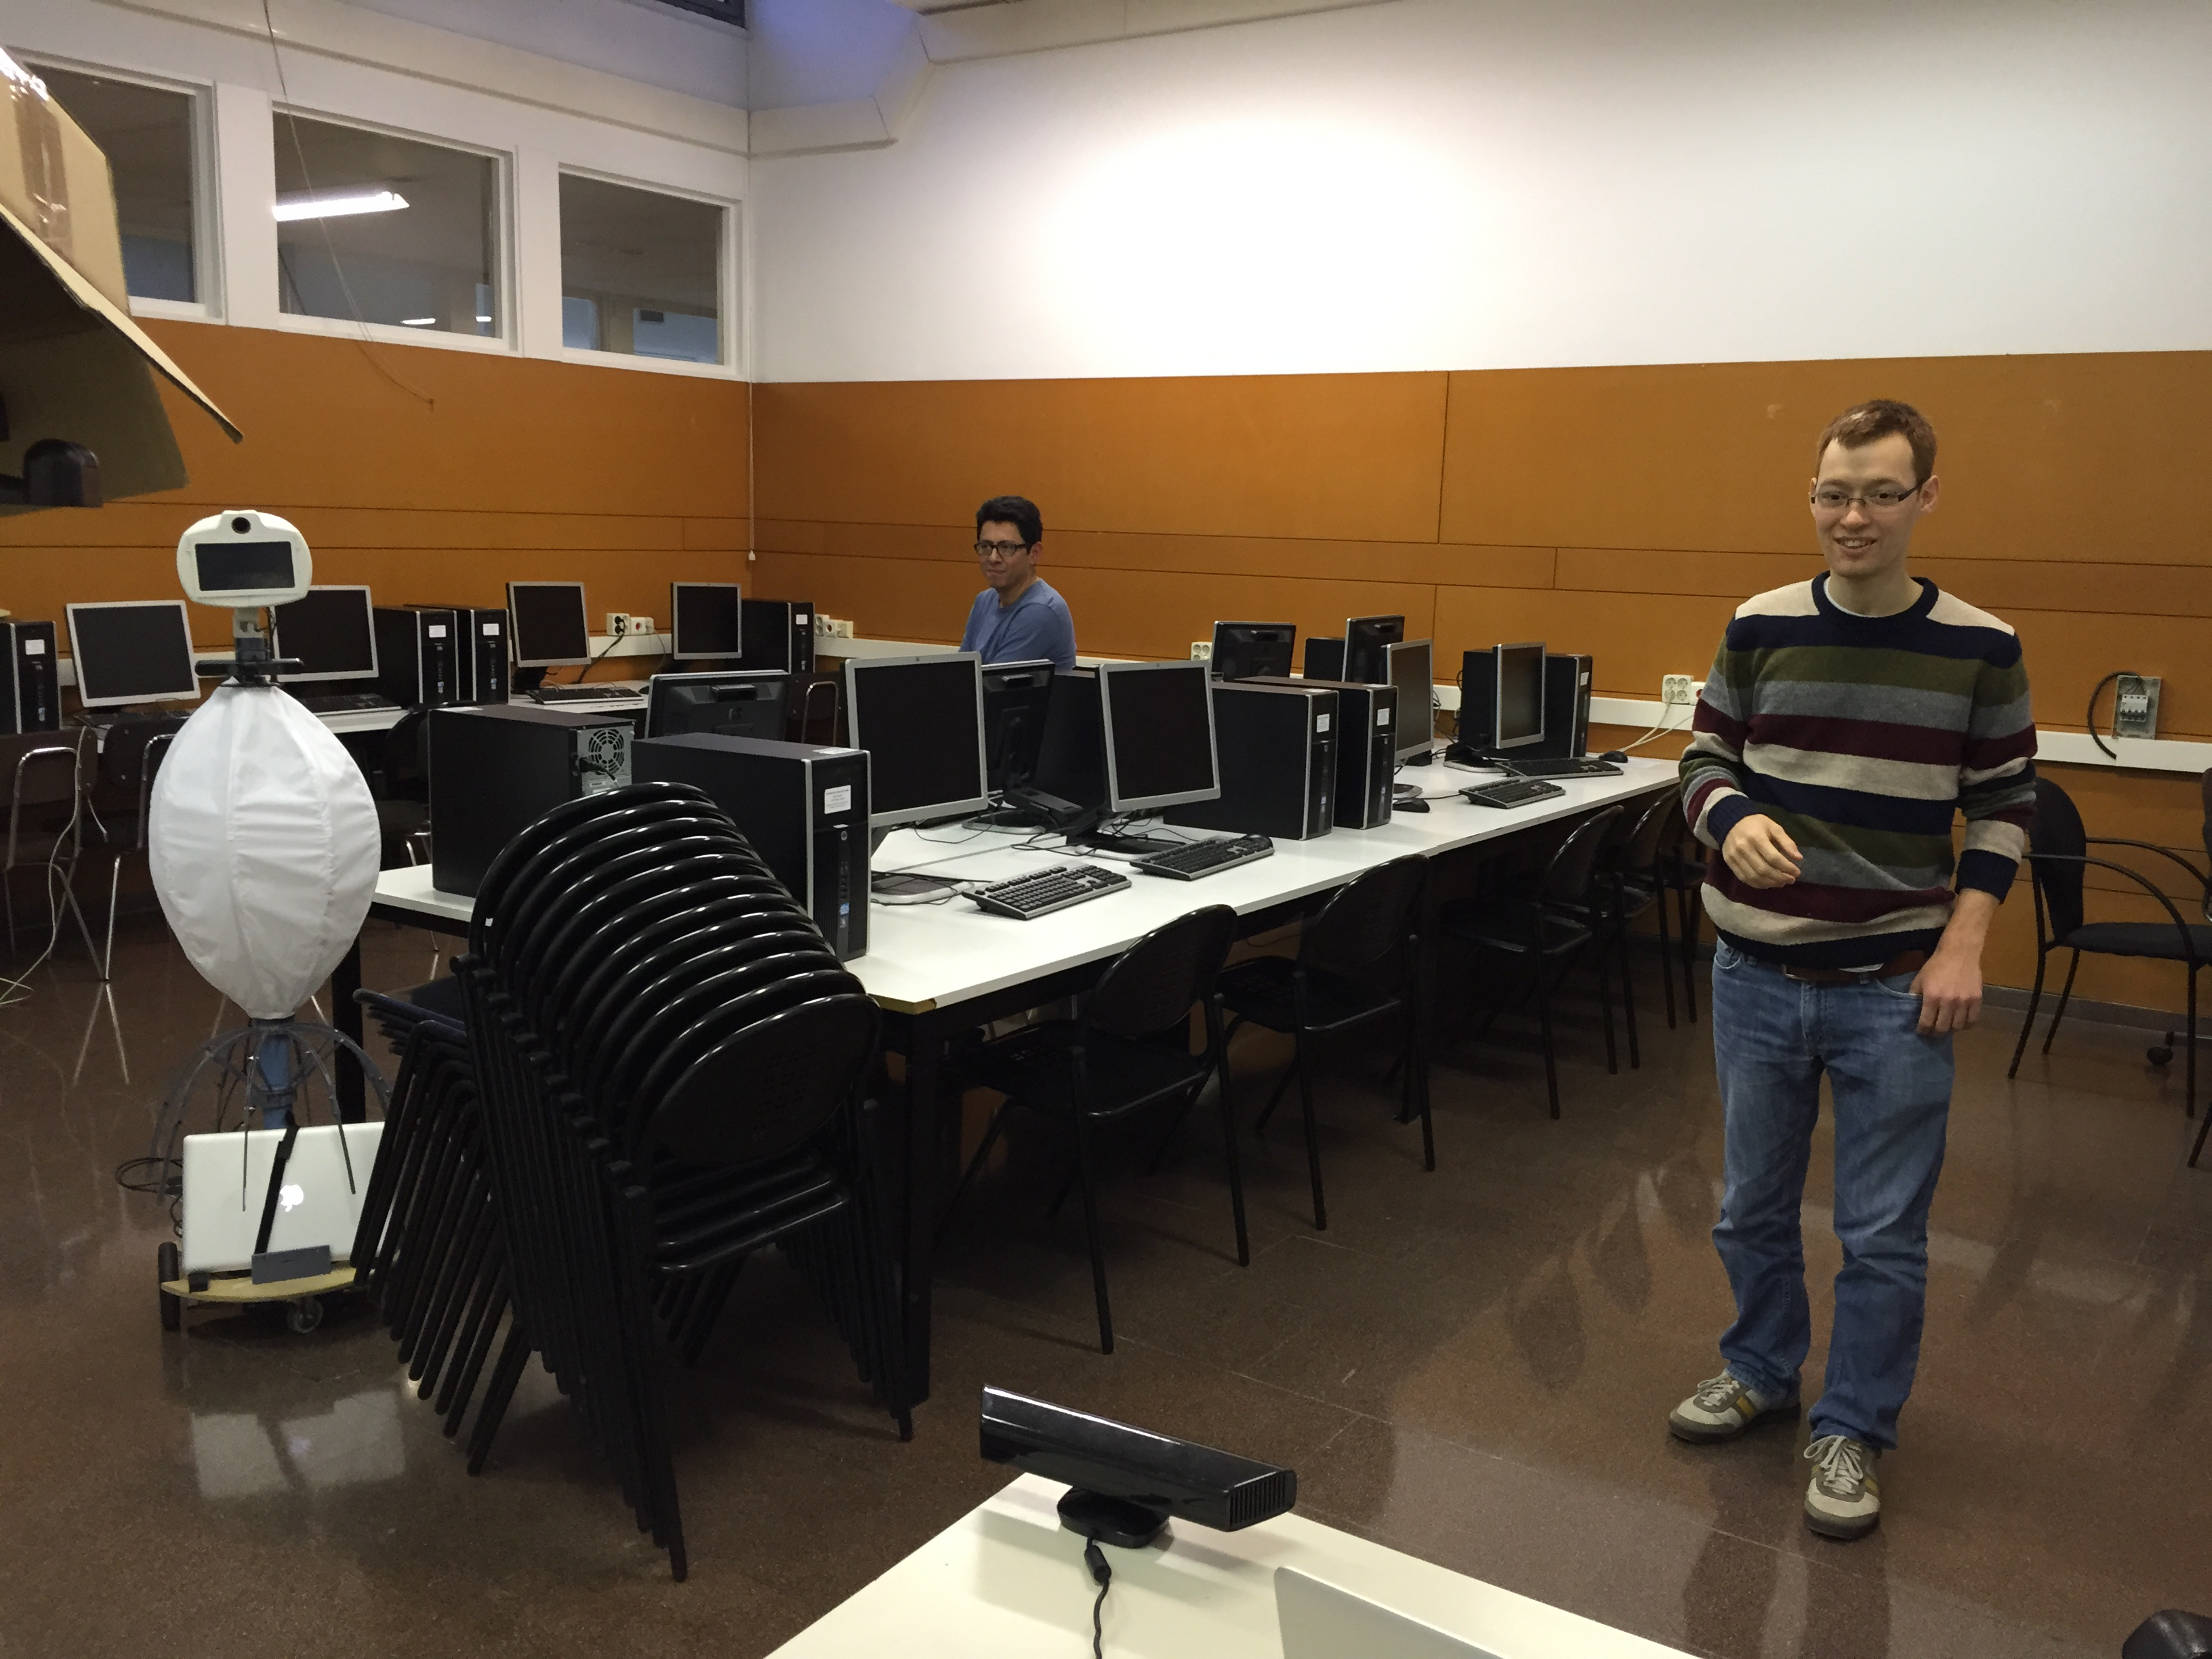
\includegraphics[width=\textwidth]{images/4_Gestures_Test.JPG}
		%\caption{Gestures Test}
		\label{fig:gest3}
	\end{subfigure}
	\caption{Gestures Test}\label{fig:gest}
\end{figure}

The results from the numerical questions in the survey where the following:

\begin{table}[h!]
	\centering
	\begin{tabular}{|l|M{3cm}|N}
		\hline
		\textbf{Questions} & \textbf{Answers} (Disagree 1 - 5 Totally Agree) \\\hline
		The system is easy to use. & $3.75 \pm 0.43$ \\
		The system is intuitive. & $4.25 \pm 0.5$ \\
		The system responds accordingly to your expectations. & $3.25 \pm 0.89$ \\
		The gesture commands are easy and intuitive. & $5 \pm 0$\\
		The anti-collision system is useful. & $4.75 \pm 0.43$\\
		\hline
	\end{tabular}
	\label{tab:survey}
\end{table}

We can see that the system in general was easy and intuitive to use and that the anti-collision system was of good use. However we can see there is more discrepancy on whether the system responded accordingly to the expectations of the testers.\\

The testers also respond all positively to the question \textit{`Do you think the speed reduction is useful?'} and agree to disagree in the question \textit{`Which gesture is more complicated to detect?'} since from the 4 answers just two of them where the same (Forward).\\

Three of the four testers agree that the stopping distance of the robot was acceptable or good (500 - 600 mm), just one of the users thought it was too close, the tester felt comfortable with a distance of 700 mm. This difference in distance could be determined by different factors but is well known that culture influences these measure, and that could be the reason why that tester felt uncomfortable since he was the only non Spanish tester.

\begin{figure}[htb!]
	\centering
	\begin{subfigure}[b]{0.3\textwidth}
		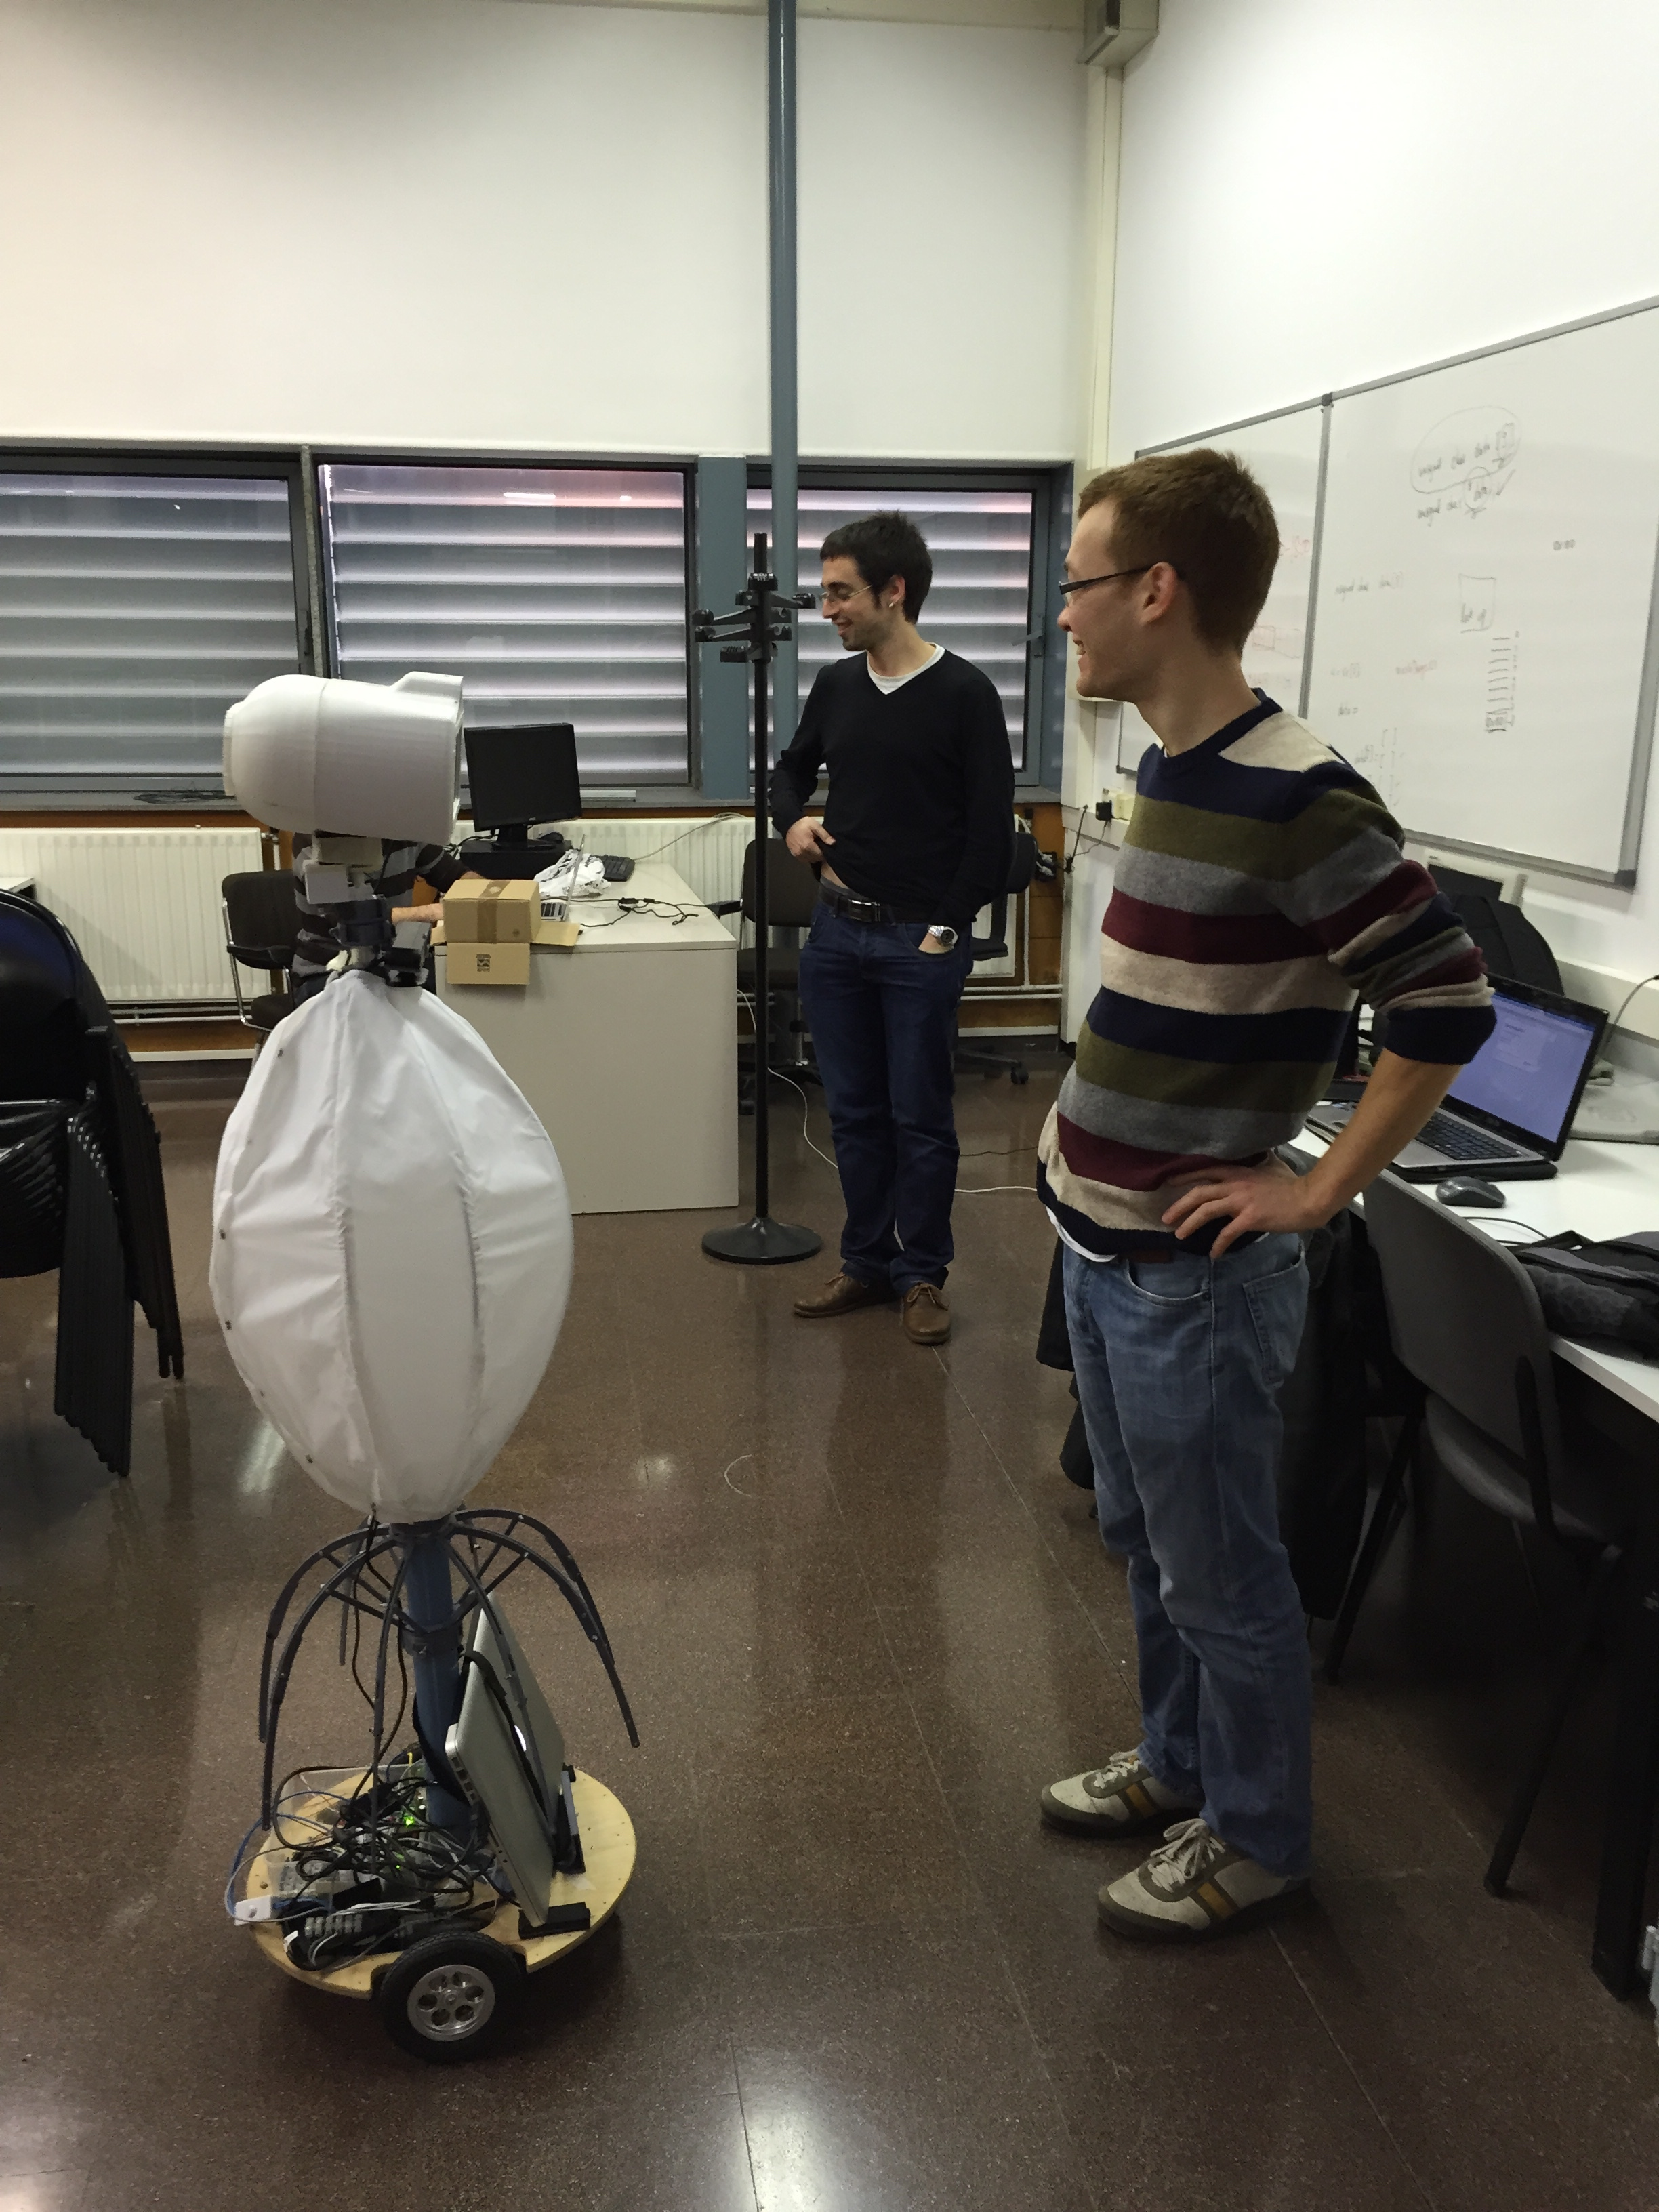
\includegraphics[width=\textwidth]{images/6_Confort_Area.jpg}
		%\caption{Comfort test 1}
		\label{fig:comf1}
	\end{subfigure}
	~ %add desired spacing between images, e. g. ~, \quad, \qquad, \hfill etc.
	%(or a blank line to force the subfigure onto a new line)
	\begin{subfigure}[b]{0.3\textwidth}
		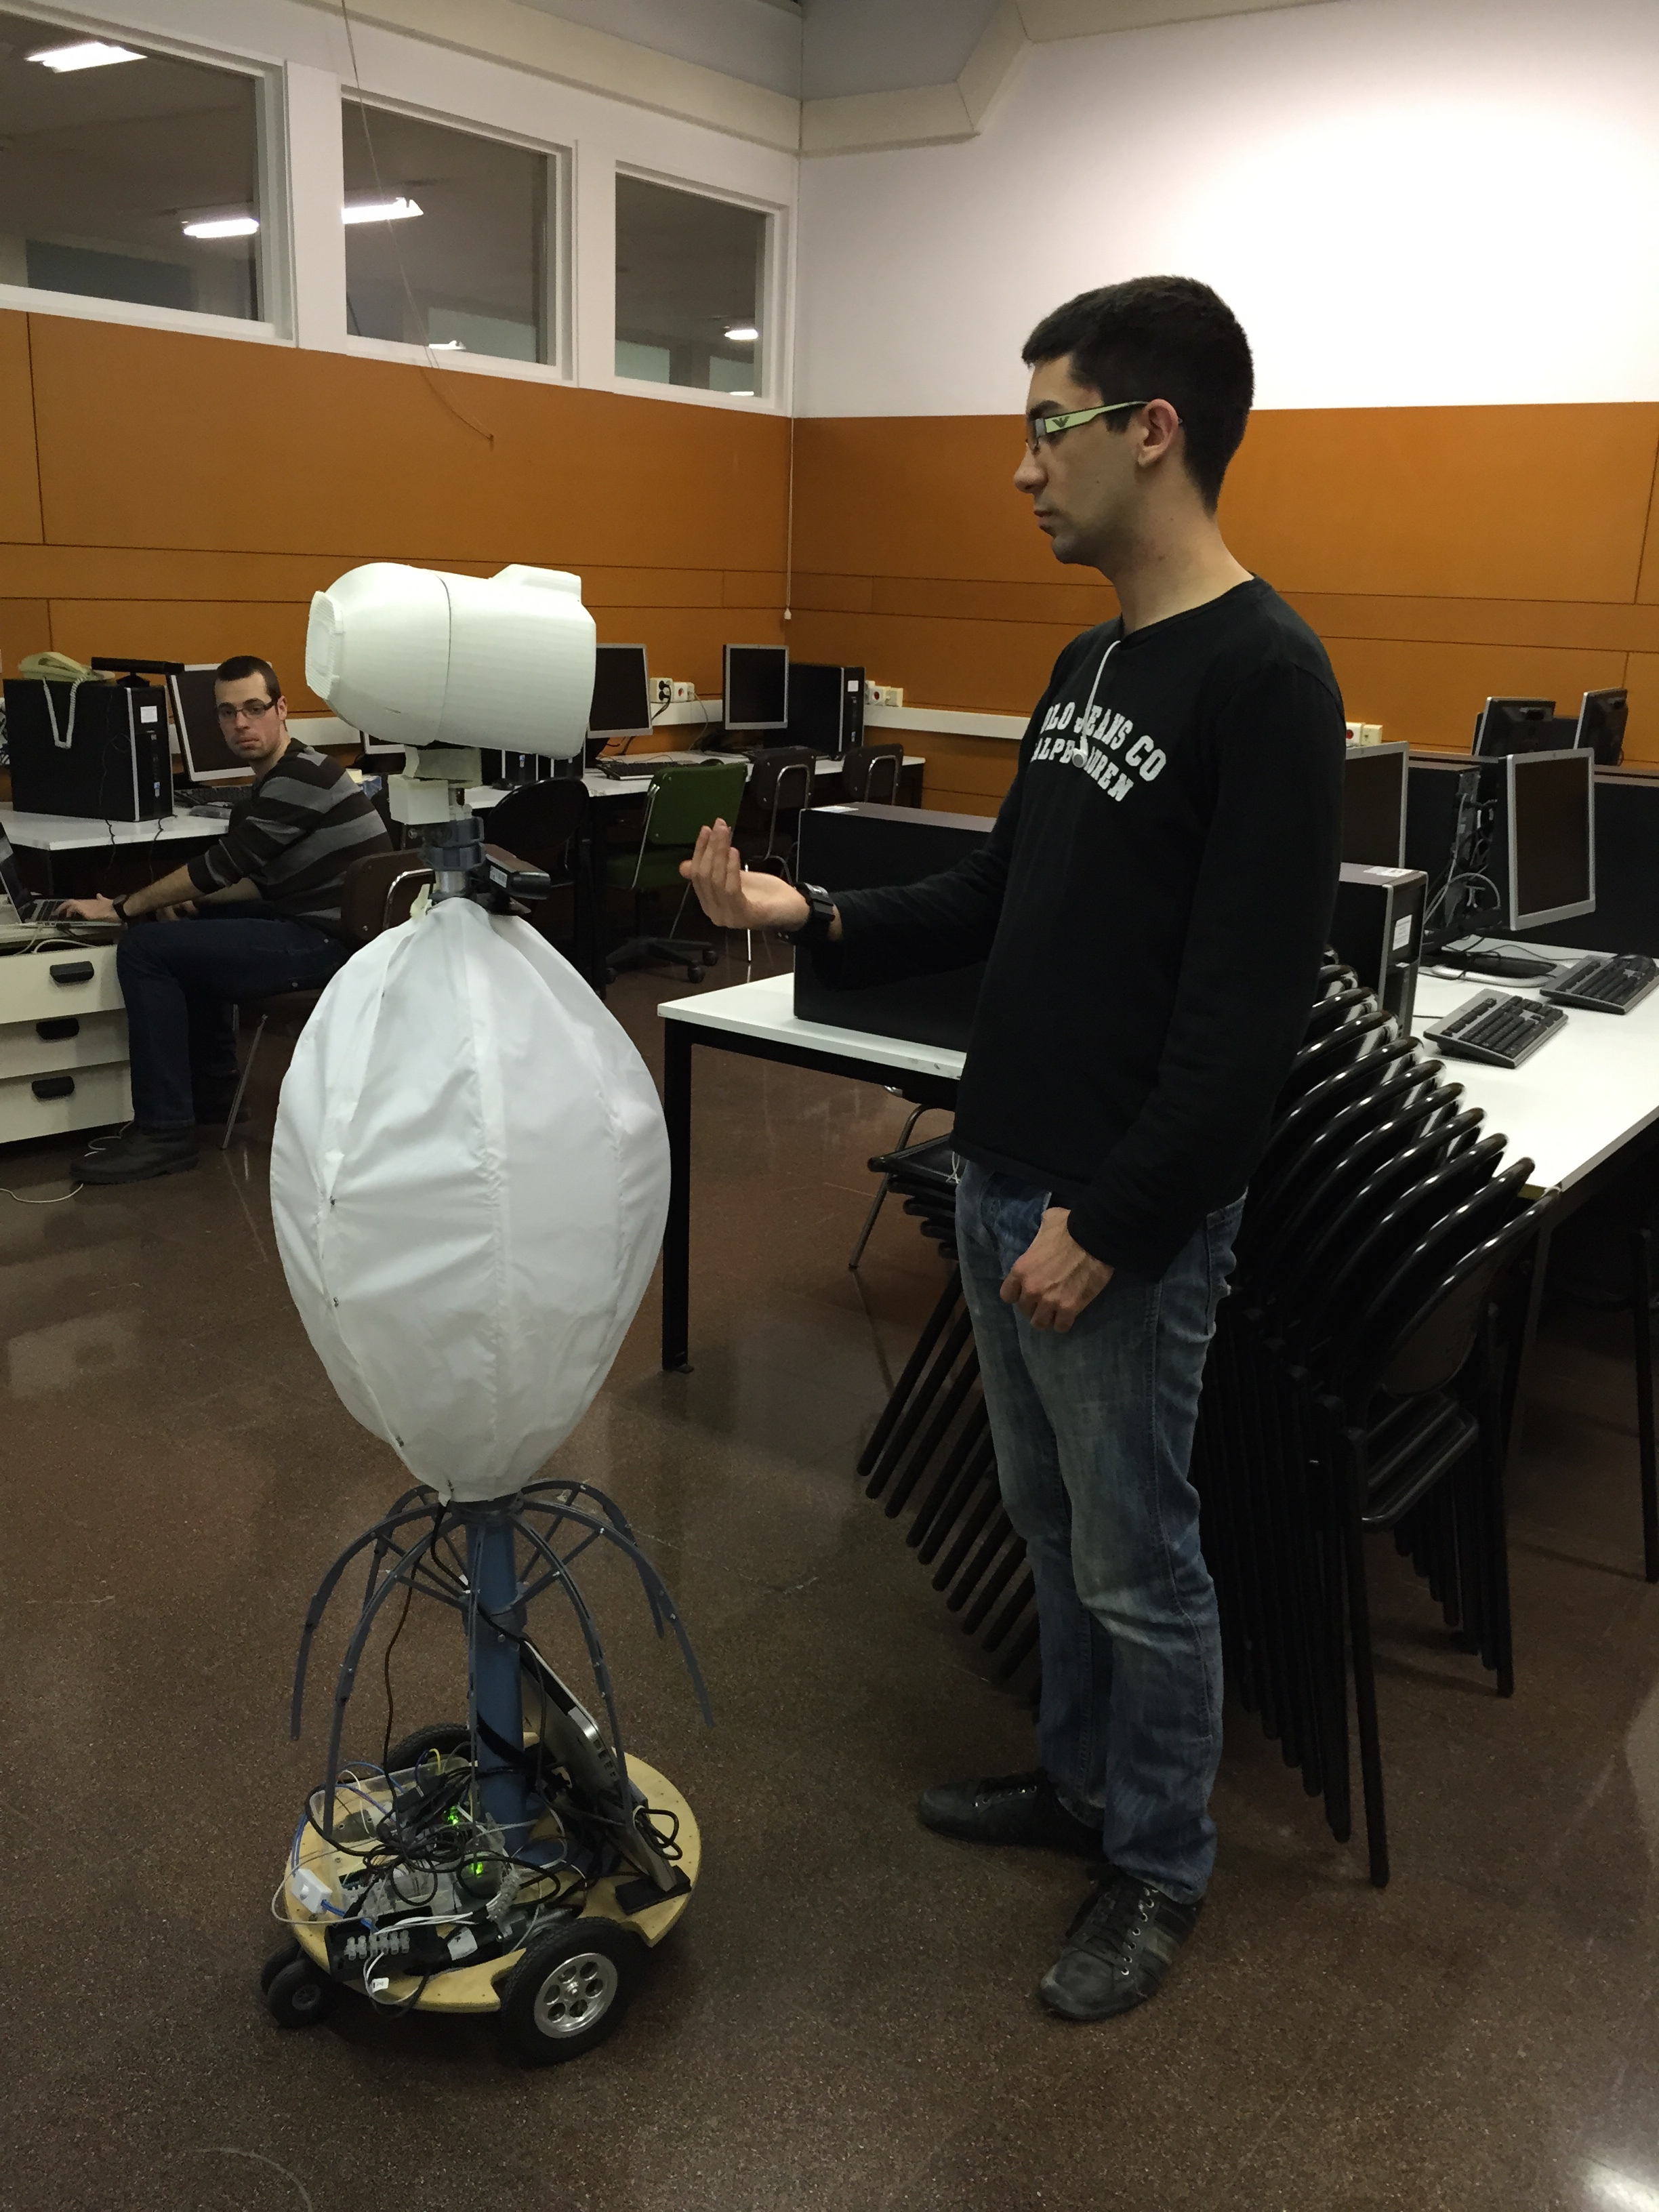
\includegraphics[width=\textwidth]{images/7_Confort_Area.jpg}
		%\caption{Comfort test 2}
		\label{fig:comf2}
	\end{subfigure}
	\caption{Comfort Test}\label{fig:comf}
\end{figure}

\begin{figure}[htb!]
	\centering
	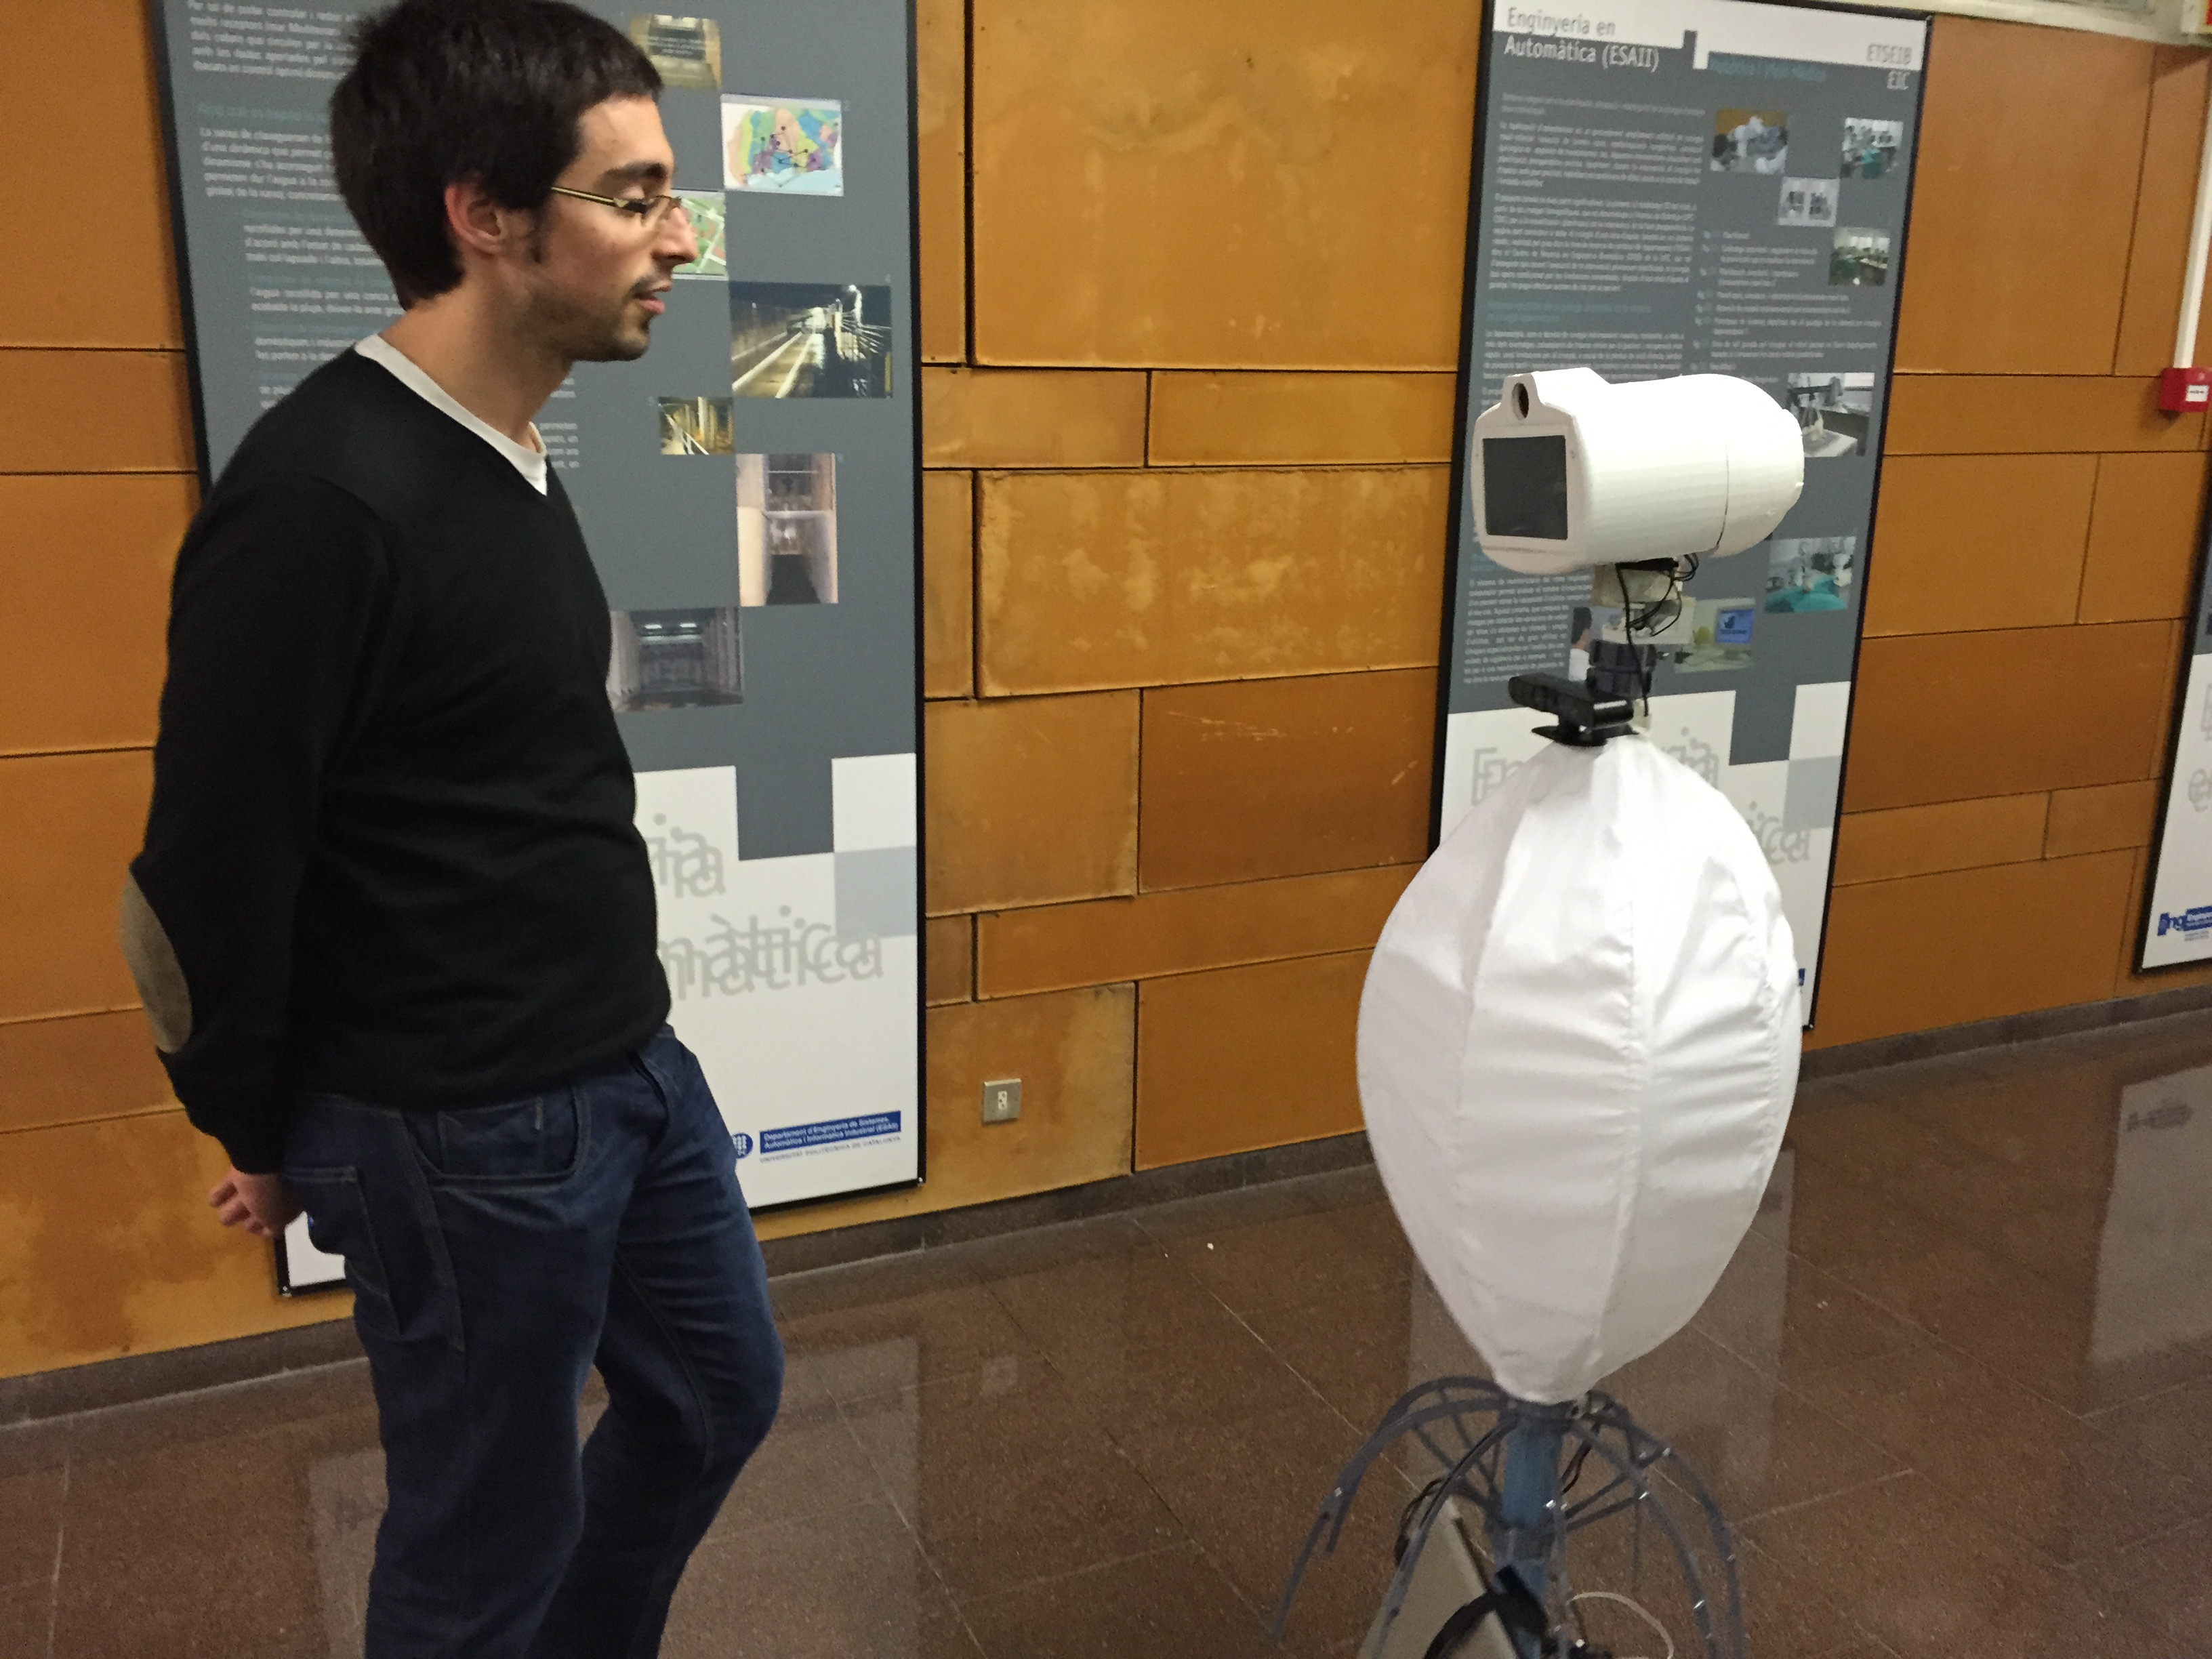
\includegraphics[width=0.5\textwidth]{images/5_Collision_Control.JPG}
	\caption{Collision Control}
	\label{fig:coll}
\end{figure}
